\section{Příklad 1}
% Jako parametr zadejte skupinu (A-H)
\prvniZadani{H}
\subsection{Výpočet $R_{ekv}$}
\begin{figure}[H]
     \centering
     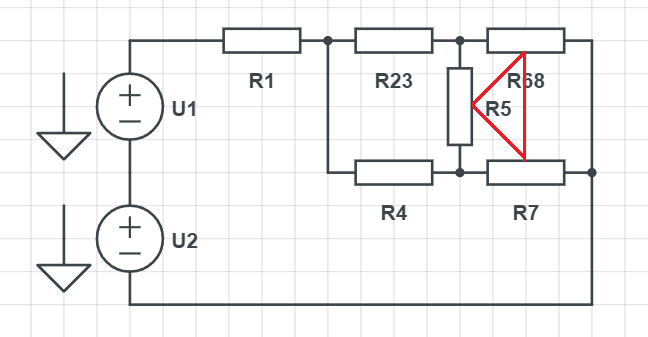
\includegraphics[scale=0.6]{pic1/u1o1.png}
     \caption{$R_2 + R_3$}
     \label{fig:Paralel_resistor_R23}
     \begin{quote}
     \centering
     $R_{23} =  \dfrac{R_2 * R_3}{R_2 + R_3} $  \\~\\
     $R_{23} =  \dfrac{600\Omega * 260\Omega}{600\Omega + 260\Omega} = 
     \dfrac{156000\Omega}{860\Omega} = 181.3953\Omega$ \\~\\
     $R_{68} =  {R_6 + R_8} $  \\~\\
     $R_{68} =  {870\Omega + 265\Omega} = {1135\Omega} $\\~\\
\end{quote}
\end{figure}
\begin{figure}[H]
    \centering
    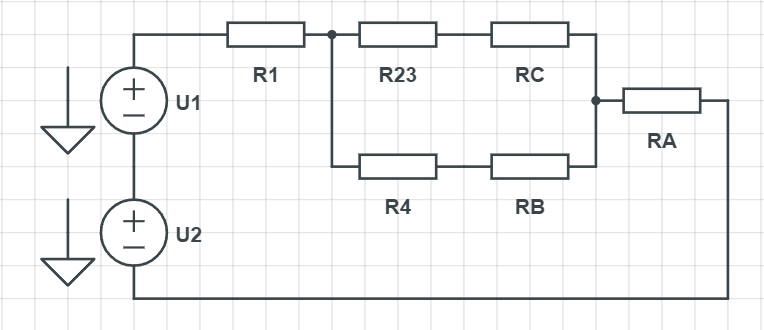
\includegraphics[scale=0.6]{pic1/u1o2.png}
    \caption{$Trojuhelnik \quad hvezda$}
    \label{fig:Trojuhelnik_Hvezda}
    \begin{quote}
    \centering
    $R_A =  \dfrac{R_{68} * R_7}{R_5 + R_{68} + R_7} $  \\~\\
    $R_B =  \dfrac{R_7 * R_5}{R_5 + R_{68} + R_7} $  \\~\\
    $R_C =  \dfrac{R_5 * R_{68}}{R_5 + R_{68} + R_7} $  \\~\\
    \medskip
    $R_A =  \dfrac{1135\Omega * 355\Omega}{575\Omega + 1135\Omega + 355\Omega} = \dfrac{402925\Omega}{2065\Omega} = 195.1210\Omega$ \\~\\
    $R_B =  \dfrac{355\Omega * 575\Omega}{575\Omega + 1135\Omega + 355\Omega} = \dfrac{204125\Omega}{2065\Omega} = 98.8498\Omega$ \\~\\
    $R_C =  \dfrac{575\Omega * 1135\Omega}{575\Omega + 1135\Omega + 355\Omega} = \dfrac{652625\Omega}{2065\Omega} = 316.0411\Omega$ \\~\\
    \end{quote}

    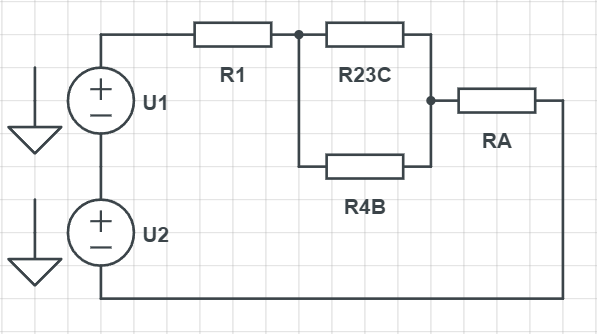
\includegraphics[scale=0.6]{pic1/u1o3.png}
    \caption{$Seriove \: zapojeni \quad R_{23} + R_C \quad a \quad R_4 + R_B $ }
    \label{fig:Serial_resistor_R23C_and_R4B}
    \begin{quote}
    \centering
    $R_{23C} = R_{23} + R_C $  \\~\\
    $R_{4B} = R_4 + R_B $  \\~\\
    $R_{23C} = 181.3953\Omega + 316.0411\Omega = 497.4364\Omega$ \\~\\
    $R_{4B} =310\Omega + 98.8498\Omega = 408.8498\Omega$ \\~\\
    \end{quote}
\end{figure}
\begin{figure}[H]
     \centering
     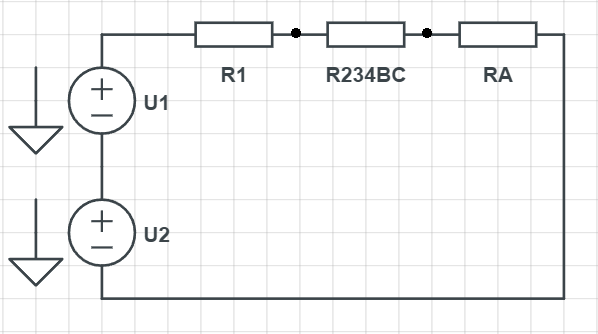
\includegraphics[scale=0.6]{pic1/u1o4.png}
     \caption{$Paralelne \: zapojene \: R_{23C} \: a \: R_{4B} \: a \: Zjednoduseni \: do \: R_{ekv}$}
     \label{fig:Paralel_resistor_R234BC}
     \begin{quote}
     \centering
     $R_{234BC} =  \dfrac{R_23C * R_4B}{R_23C + R_4B} $  \\~\\
     $R_{234BC} =  \dfrac{497.4364\Omega * 408.8498\Omega}{497.4364\Omega + 408.8498\Omega} = 
     \dfrac{203376.7726\Omega}{906.2862\Omega} = 224.4067\Omega$ \\~\\
\end{quote}
    \label{fig:REKV}
    \begin{quote}
    \centering
    $R_{ekv} = R_{1234ABC} = R_1 + R_{234BC} + R_A$  \\~\\
    $R_{ekv} = R_{1234ABC} = 680\Omega + 224.4067\Omega + 195.1210\Omega = 1099.5279 \Omega $  \\
    \end{quote}
    S $R_{ekv}$ nyní můžeme vypočítat celkový proud v obvodu Ohmovým zákonem: $I = \dfrac{U}{R_{ekv}}$
    \begin{quote}
    \centering
    $U = U_1 + U_2$ \\~\\
    $U = 135\Vo + 80\Vo = 215\Vo$ \\~\\
    $I = \dfrac{215\Vo}{1099.5279\Omega} = 0.0266\Am$
    \end{quote}
\end{figure}
    \subsection{Výpočet $U_{R2}$}
    \begin{quote}
    \centering
	Rozložíme zpětně obvod \\~\\
	$U_{R234BC} = I * R_{234BC}$ \\~\\
	$U_{R234BC} = 0.0266\Am * 224.4067\Omega = 43.8801\Vo$ \\~\\
    \end{quote}




\begin{figure}[H]
    \centering
    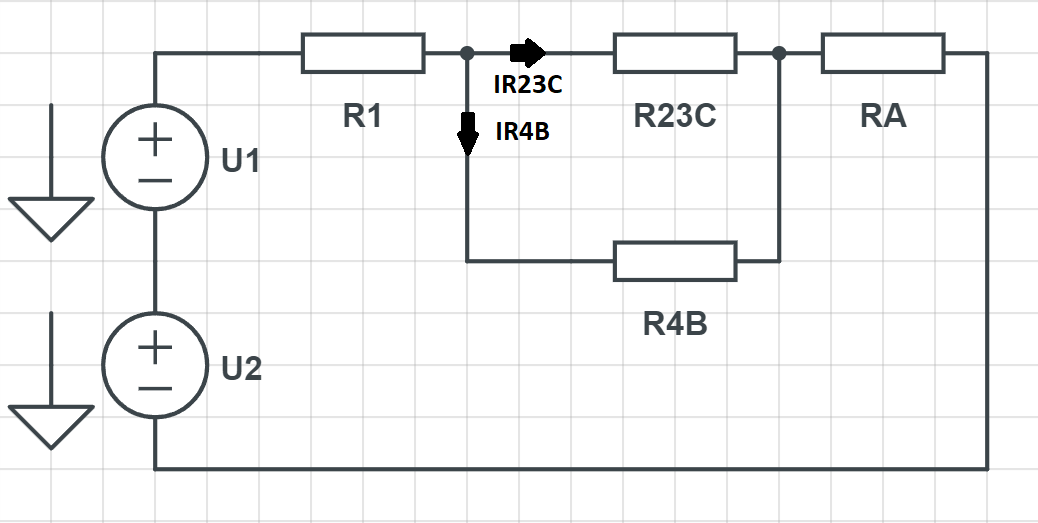
\includegraphics[scale=0.45]{pic1/u1o5.png}
    \begin{quote}
    \centering
    $I_{R23C} = \dfrac{U_{R2346BC}}{R_{23C}} $ \\~\\
	$I_{R23C} = \dfrac{43.8801\Vo}{497.4364\Omega} = 0.0882\Am $ \\~\\
    \end{quote}
\end{figure}
\begin{figure}[H]
    \centering
    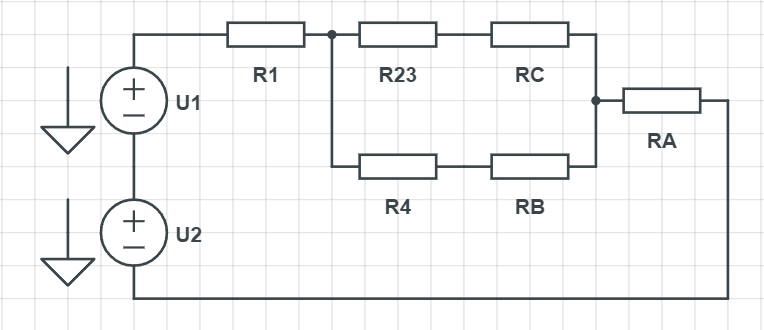
\includegraphics[scale=0.6]{pic1/u1o6 .png}
    \begin{quote}
    \centering
    $I_{R23} = I_{R23C}$ \\~\\
	$U_{R23} = I_{R23}*R_{23} $ \\~\\
	$U_{R23} = 0.0882\Am * 181.3953\Omega = 16.0016\Vo $ \\~\\
    \end{quote}
\end{figure}
\begin{figure}[H]
    \centering
    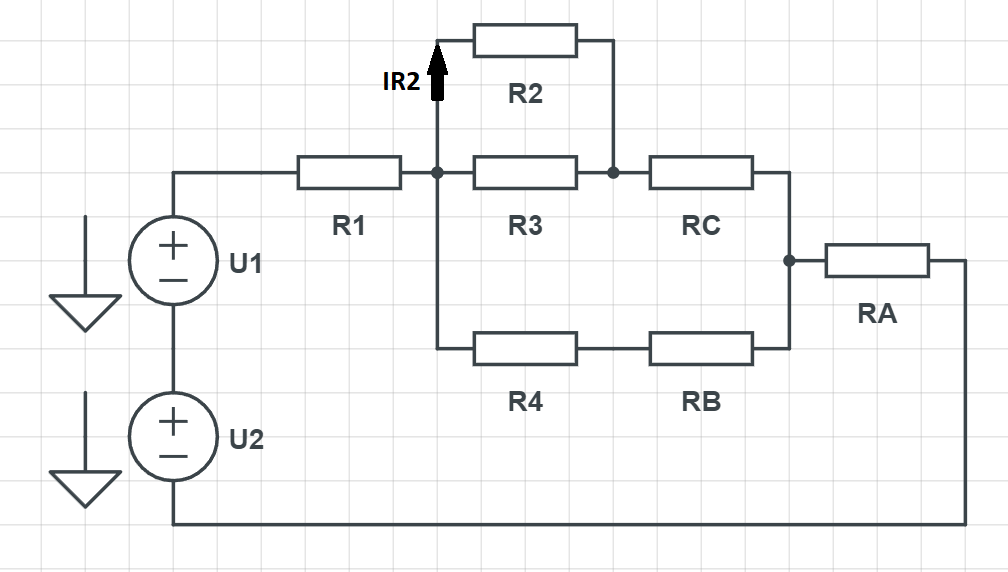
\includegraphics[scale=0.45]{pic1/u1o7.png}
    \begin{quote}
        \centering
         $U_{2} = U_{23} = 16.0016\Vo $ \\~\\
         $I_{R2} = \dfrac{U_{R23}}{R_{2}}$ \\~\\
         $I_{R2} = \dfrac{16.0016\Vo}{600\Omega} = 0.0266\Am$ \\~\\
    \end{quote}
\end{figure}
